\documentclass[%
 preprint,
 amsmath,amssymb,
 aps,
]{revtex4-2}

\usepackage{graphicx}
\graphicspath{{figures/}}

\usepackage{physics}
\usepackage{siunitx}

\newcommand{\vf}{v_{\mathrm{F}}}
\newcommand{\qf}{q_{\mathrm{F}}}
\newcommand{\pf}{p_{\mathrm{F}}}
\newcommand{\epsF}{\epsilon_{\mathrm{F}}}
\newcommand{\debye}{\omega_{\mathrm{D}}}
\newcommand{\corr}{\mu^{\ast}}
\newcommand{\dof}{\rho}
\usepackage{cleveref}

\begin{document}

\title{Evanescent-wave Johnson noise from BCS superconductors}

\author{Hruday Mallubhotla}
\author{Robert Joynt}
 \email{rjjoynt@wisc.edu}
\affiliation{
 Physics Department, University of Wisconsin-Madison\\
1150 University Ave, Madison, WI 53706, USA
}

\date{\today}

% TODO: write abstract after finished up with everything else
%\begin{abstract}
%\end{abstract}

\maketitle

\tableofcontents

\section{Intro} \label{sec:intro}

In the current paper, we use the superconducting dielectric function discussed by Nam\cite{Nam1967}, for the special case of a weak-coupling superconductor with only non-magnetic impurities.
We also describe methods of obtaining results in the momentum regime where this dielectric function ceases to be valid.
The relaxation times for a qubit outsied a typical BCS superconductor are discussed.
In particular, we look at the relationship between transition temperature and frequency between a low-noise superconducting state and a high-noise normal state.
Additionally, we extend this dielectric function to model non-equilibrium quasiparticle poisoning via a method discussed by Owen and Scalapino\cite{OwenScalapino}.
We then look at the effect of this poisoning on relaxation times.

\section{Equilibrium state} \label{sec:equilibrium}
\subsection{Qubit Relaxation Time Formalism} \label{subsec:relaxtime}
Physically, we are interested in the relaxation time of a qubit near the surface of the metal.
Sufficiently close to the metal, such that the separation between qubit and metal is much smaller than the shortest dimension of the metallic body, we can approximate the metal as a half space.
This defines a natural coordinate system, and we can allow the metal to take up all points with $z$-coordinate less than zero, extending to infinity in the $x$ and $y$ directions.

For a charge qubit with level separation $\omega$ and dipole moment $\vec{d}$, the relaxation rate $\frac{1}{T_1}$ depends on the qubit's distance from the surface $z$, as well as its orientation $i$.
The vacuum wavelength $\lambda = \frac{c}{\omega}$ is a natural unit for this distance $z$, so we wil measure $z$ in units of $\lambda$.
The electromagnetic field fluctuations that contribute to qubit relaxation have been described in~\cite{QubitRelax} and~\cite{Henkel1999}.
Both use Fermi's golden rule and the fluctuation-dissipation theorem to relate the relaxation rate to the spectral density of the field fluctuations, and obtain the following expression:
\begin{equation}
	\frac{1}{T_1} = \frac{d^2}{\epsilon_0} \frac{\omega^3}{c^3} \chi_{i}^{(E)}(z, \omega) \coth\frac{\omega}{2 T}.
\end{equation}
%Here and elsewhere we take $\hbar = k_{\mathrm{B}} = 1$.

Similarly, for spin qubits with dipole moment $\vec{\mu}$, both~\cite{QubitRelax} and~\cite{Henkel1999} have a similar expression with a different spectral density expression:
\begin{equation}
	\frac{1}{T_1} = \frac{\mu^2}{\epsilon_0} \frac{\omega^3}{c^3} \chi_{i}^{(B)}(z, \omega) \coth\frac{\omega}{2 T}.
\end{equation}

\subsubsection{Spectral Field Densities} \label{subsec:spectraldensities}
The spectral densities are in general functions of the geometry and electrodynamic response of the metal object.
A standard limiting case for the response is that of local, linear electrodynamics, where the relationship between the electric displacement $\vec{D}$ and electric field $\vec{E}$ is a proportionality:
\begin{equation}
	\vec{D}(\vec{r}) = \epsilon \vec{E}(\vec{r})
\end{equation}
For a metal with conductivity $\sigma$, this dielectric function will typically have a large imaginary value as determined by the Drude expression in Gaussian units:
\begin{equation}
	\epsilon = 1 + i\frac{4 \pi \sigma}{\omega}
\end{equation}

For a half space, these spectral densities can be written in terms of the surface's reflection coefficients, as derived by\cite{Henkel1999} for local electrodynamics.
Considering for now a qubit pointing in the direction perpendicular to the half-space, we can write
\begin{align}
	\chi_\perp^E(z, \omega) &= \Re \int_0^{+\infty} \dd{u} \frac{u^3}{v} e^{2 i z v} r_p(u). \label{eq:chi}
\end{align}
The integration variable $u$ effectively represents a momentum in units of $\flatfrac{1}{\lambda}$, with $v = \sqrt{1 - u^2}$.
If $v \geq 1$, we take the positive square root $v = i \sqrt{u^2 - 1}$.
The magnetic spectral density is the same, except with an additional factor of $\flatfrac{1}{c^2}$ and with $r_s$ instead of $r_p$.
In the local limit, for dielectric constant $\epsilon$, the reflection coefficients will be the Fresnel $r_p$ and $r_s$:
\begin{align}
	r_p &= \frac{\epsilon v - \sqrt{\epsilon - u^2}}{\epsilon v + \sqrt{\epsilon - u^2}} \\
	r_s &= \frac{v - \sqrt{\epsilon - u^2}}{ v + \sqrt{\epsilon - u^2}}
\end{align}

\subsubsection{Nonlocal Electrodynamics} \label{subsubsec:nonlocalelectrodynamics}
However, as discussed in~\cite{QubitRelax} and~\cite{Henkel2006}, this expression no longer remains accurate for arbitrarily small distances, with \eqref{eq:chi} diverging as $\frac{1}{z^3}$ as $z \rightarrow 0$.
The divergence here stems from the unphysicality of local electrodynamics at very small scales;
for $z$ smaller than the electromagnetic coherence length of the metal the full response function defined by
\begin{equation}
	\vec{D}(\vec{r, t}) = \int \dd{r'} \dd{t'} \epsilon(r, r', t, t') \vec{E}(\vec{r', t'})
\end{equation}
becomes necessary.
The experiment described by Kolkowitz et al.\cite{Kolkowitz2015} gives an example of a physical situation where the local description is insufficient, with a qubit probe at a distance from a silver film less than the film's mean free path.
Given that the coherence lengths of typical BCS superconductors can be larger than the distances used in that experiment, we should expect that the purely local description will not work for the superconducting case.

To keep~\eqref{eq:chi} accurate for sufficiently small $z$, appropriate changes to the reflection coefficients can be made\cite{QubitRelax,Henkel2006} through the reflection coefficients in Ford and Weber~\cite{Ford1984}:
\begin{align}
	r_p(u) &= \frac{\pi v - \zeta_p(u)}{\pi v + \zeta_p(u)} \\
	r_s(u) &= \frac{\zeta_s(u) - \frac{\pi}{v}}{\zeta_s(u) + \frac{\pi}{v}} \\
	\zeta_p(u) &= 2i \int_0^\infty \dd{y} \frac{1}{\kappa^2} \left( \frac{y^2}{\epsilon(\frac{\omega}{c}\kappa, \omega) - \kappa^2} + \frac{u^2}{\epsilon_(\frac{\omega}{c}\kappa, \omega)} \right) \label{eq:zp} \\
	\zeta_s(u) &= 2i \int_0^\infty \dd{y} \frac{1}{\epsilon(\frac{\omega}{c}\kappa, \omega) - \kappa^2} \label{eq:zs} \\
	\kappa^2 &= u^2 + y^2
\end{align}
The quantities $\zeta_p$ and $\zeta_s$ are proportional to the surface impedances of the metal, derived for this case by Ford and Weber\cite{Ford1984}, and with more thorough discussion in~\cite{LandauLifshitzElectrodynamics}.
The treatment in~\cite{QubitRelax} compares the difference between these expressions and the simpler Fresnel reflection coefficients.

\subsection{Dielectric Function} \label{subsec:dielectric}
\subsubsection{Normal state dielectric function} \label{subsubsec:lindharddielectric}
The dielectric function $\epsilon(q, \omega)$, then, contains the information needed to describe the electromagnetic properties of the surface near the qubit.
For the normal state, the dielectric function derived by Lindhard~\cite{Lindhard} used in~\cite{QubitRelax} describes the non-local electromagnetic response of a metal.
Using the form described by Solyom\cite{SolyomV3},
\begin{equation}
	\epsilon_{\mathrm{Lindhard}}(\vec{q}, \omega) = 1 + \frac{q_{TF}^2}{q^2}\frac{\displaystyle 1 + \frac{\omega + \flatfrac{i}{\tau}}{2 \vf q} \ln(\frac{\omega - \vf q + \flatfrac{i}{\tau}}{\omega + \vf q + \flatfrac{i}{\tau}})}{\displaystyle 1 + \frac{\flatfrac{i}{\tau}}{2 \vf q} \ln(\frac{\omega - \vf q + \flatfrac{i}{\tau}}{\omega + \vf q + \flatfrac{i}{\tau}})}. \label{eq:lindhardsolyom}
\end{equation}
Here, $q_{TF}$ is the Thomas-Fermi wavevector $q_{TF}^2 = 3 \flatfrac{\omega_p^2}{\vf^2}$, $\omega_p$ is the plasma frequency $\sqrt{\flatfrac{4 \pi n e^2}{m}}$, $\tau$ is the collision time and $\vf$ is the Fermi velocity.
The branch cut for the logarithm is chosen here such that their imaginary parts lie between $\pm i \pi$.
This can be shown to reduce to the Drude dielectric function in the $q \rightarrow 0$ limit.

The Lindhard dielectric function reflects the important property of having an imaginary part that vanishes for $q$ such that $\abs{\varepsilon_q - \omega} >  q\vf$.
This is a very generic feature of these types of response functions, and occurs because there are no points on the assumed spherical Fermi surface further than $2 q_{\mathrm{F}}$ apart.
Thus, there are no available quasiparticle-hole excitations available for energy dissipation (cf discussion in \cite{AGD}, \cite{FetterWalecka} or \cite{SolyomV3}).
This is a general argument, and it should be expected that a superconducting dielectric function should also have zero imaginary part above some momentum on the order of the Fermi momentum.
Because the Lindhard dielectric function's imaginary part vanishes above a cutoff $q_c\left(\omega\right)$ and has real part that goes as $\Re \epsilon_{\mathrm{Lindhard}} - 1 \sim \frac{1}{q^2}$, all of the integrals in $\eqref{eq:chi}, \eqref{eq:zp} and \eqref{eq:zs}$ converge.

\subsubsection{Superconducting dielectric function} \label{subsubsec:namdielectric}

We use the expressions from Nam in~\cite{Nam1967} to represent the superconducting response function.
This extends the previous models by Mattis and Bardeen~\cite{Mattis} and Abrikosov, Dzyaloshinskii and Gorkov\cite{AGD} to give expressions that allow for broader ranges of impurity values.

Here, we look at Nam's expressions in the weak coupling limit, for no magnetic impurities and an isotropic material.
\begin{equation}
	\epsilon_{\mathrm{Nam}}(\vec{q}, \omega) = 1 + \frac{3 \pi}{\omega^2} \frac{n e^2}{m} \left[\int_{\Delta - \omega}^{\Delta}\dd{\omega'} \tanh(\frac{\omega + \omega'}{2 T}) I_1 + \int_{\Delta}^{\infty} \dd{\omega'} \left( \tanh(\frac{\omega + \omega'}{2 T}) I_1  - \tanh(\frac{\omega'}{2 T})I_2 \right) \right], \label{eq:eps}
\end{equation}
with
\begin{align}
	I_1 &= F(q, \Re[\sqrt{(\omega + \omega')^2 - \Delta^2} - \sqrt{\omega'^2 - \Delta^2}]) (g + 1) \nonumber\\
	&\quad + F(q, \Re[-\sqrt{(\omega + \omega')^2 - \Delta^2} - \sqrt{\omega'^2 - \Delta^2}]) (g - 1) \\
	I_2 &= F(q, \Re[\sqrt{(\omega + \omega')^2 - \Delta^2} - \sqrt{\omega'^2 - \Delta^2}]) (g + 1) \nonumber\\
	&\quad + F(q, \Re[\sqrt{(\omega +  \omega')^2 - \Delta^2} + \sqrt{\omega'^2 - \Delta^2}]) (g - 1) \\
	F(q, E) &= \frac{1}{q \vf} \left[2 S(E) + (1 - S(E)^2)\ln(\frac{S(E) + 1}{S(E) - 1})\right] \label{eq:NamF} \\
	S(q, E) &= \frac{1}{q \vf} \left( E - i \left(\Im[\sqrt{(\omega + \omega')^2 - \Delta^2} + \sqrt{\omega'^2 - \Delta^2}] + \frac{2}{\tau} \right) \right) \\
	g &= \frac{\omega' \left(\omega + \omega'\right) + \Delta^2}{\sqrt{\omega'^2 - \Delta^2}\sqrt{(\omega + \omega')^2 - \Delta^2}}.
\end{align}
The assumption of isotropy suppresses the $q$ dependence for $\Delta$, which then is just a function of temperature, and can be described using the well-known BCS expression $\Delta \approx 3.06 \sqrt{T_c(T_c - T)}$ (see for example \cite{Tinkham}).

\begin{figure}[htp]
	\centering
	\includegraphics[width=\linewidth]{Cond1Re}
	\caption{$\Re[\epsilon(q)]$ for $\omega = 1$, $\tau = 0.5$, $\omega_p = 10$, $\vf = 1$, $T = .9999 T_c$, $T_c = 3$} \label{fig:cond1Re}
\end{figure}

\begin{figure}[htp]
	\centering
	\includegraphics[width=\linewidth]{Cond1Im}
	\caption{$\Im[\epsilon(q)]$ for $\omega = 1$, $\tau = 0.5$, $\omega_p = 10$, $\vf = 1$, $T = .9999 T_c$, $T_c = 3$} \label{fig:cond1Im}
\end{figure}

The Lindhard and Nam dielectric constants are compared in \cref{fig:cond1Re} and \cref{fig:cond1Im}, plotting the real and imaginary part for small representative values.
In this regime, $\omega_p > T_c > \omega$, as is typical for the frequency regime of interest, while $\tau$ is chosen to be smaller than $\omega$.
For a typical metal in this description, the Fermi wavevector $\qf$ is around the same order as $\sqrt{3}\frac{\omega_p}{\vf}$ (see discussion on this point in Solyom\cite{SolyomV3}).
We can see in \cref{fig:cond1Im} that the Lindhard dielectric function goes to zero for $q < \qf \approx 10 \sqrt{3}$.

\subsection{Numerical Techniques \label{subsec:technical}}

\subsubsection{Small momentum limit} \label{subsubsec:smallq}
The noise integral \eqref{eq:chi} can be calculated numerically, with proper care taken to handle the integrand's behaviour across the entire range.
For small momenta, where $\vf q \ll \omega$, both \eqref{eq:lindhardsolyom} and \eqref{eq:eps} can be series expanded to give explicit expressions.
Additionally, this small momentum limit is important in general as it tends towards the purely local limit.
The Lindhard dielectric function, up to order $q^2$, becomes
\begin{gather}
	\epsilon_{\mathrm{Lindhard}}(\vec{q}, \omega) = 1 - \frac{\omega_p^2}{\omega^2} \left(\frac{\omega}{(\omega + \frac{i}{\tau})} + (\vf q)^2  \frac{9 \omega + 5 \frac{i}{\tau}}{15 (\omega + \frac{i}{\tau})^3} \right). \label{eq:lindhardsmallkseries}
\end{gather}
As expected for a description of the normal state, for $q \rightarrow 0$ this reduces to the Drude expression.

For the superconducting case, all of the momentum dependence in the Nam expression is contained within the $F(q, E)$ function in \eqref{eq:NamF}.
Expanding this out to second order in the momentum gives
\begin{align}
	F = \frac43 \frac{1}{\eta} + (\vf q)^2\frac{4}{15} \frac{1}{\eta^3},
\end{align}
where
\begin{equation}
	\eta = E - i \left(\Im[\sqrt{(\omega + \omega')^2 - \Delta^2} + \sqrt{\omega'^2 - \Delta^2}] + 2 \frac{1}{\tau} \right).
\end{equation}
This, and other limiting forms, were stated by Nam as well~\cite{Nam1967}.
Inserting this in $\eqref{eq:NamF}$ suffices to obtain the small $q$ values in a more numerically stable way.

\subsubsection{Large momentum limit} \label{subsubsec:bigq}
By comparison, the large momentum dependence is more involved to correctly handle.
If we look at the portion of the integral in \eqref{eq:chi} for $u > u_l \gg 1$,
\begin{align}
	\chi_{\perp\ \mathrm{upper}}^E(z, \omega) &= \Re \int_{u_l}^{+\infty} \dd{u} \frac{u^3}{v} e^{2 i z v} r_p(u) \\
	\chi_{\perp\ \mathrm{upper}}^E(z, \omega) &= \Re \int_{u_l}^{+\infty} \dd{u} \frac{u^3}{i u} e^{-2 z u} r_p(u)
\end{align}
which means that for $z = 0$
\begin{align}
	\chi_\perp^E(z, \omega) &= \int^{+\infty} \dd{u} u^2 \Im r_p(u).
\end{align}
In order for this to converge, $\Im r_p(u)$ must decrease faster than $\frac{1}{u^3}$

This divergence is discussed for the normal state in Langsjoen et al.~\cite{QubitRelax}, where it only occurs in local electrodynamics.
This is related to the point earlier that the imaginary part of $\epsilon$ should go to zero for $\abs{\varepsilon_q - \omega} > q \vf$, as such a condition is sufficient to ensure that $\Im r_p(u)$ decays quickly enough.

\subsubsection{Superconducting large momentum limit} \label{subsubsec:scbigq}
The superconducting case in the large momentum limit is not automatically corrected by using nonlocal expressions, however.
For sufficiently large $q$, the logarithm in $\eqref{eq:NamF}$ goes to $i \pi$, and $F \rightarrow \frac{i \pi}{q \vf}$.
This behaviour leads to an unphysical divergence in \eqref{eq:chi} as $z \rightarrow 0$.
Tinkham~\cite{Tinkham} and Abrikosov, Dzyaloshinskii and Gorkov~\cite{AGD} both describe expressions with this same $\frac{1}{q}$ dependence.
The root cause of inaccuracies above $q \gg 2 q_{\mathrm{F}}$ is that the Green's function method used to derive the superconducting response function makes the assumption that $q$ is sufficiently close to the Fermi surface.

However, it is insufficient to only account for the $\frac{1}{q}$ dependence, as a stronger condition is necessary to ensure convergence for arbitrarily small $z$.

For a dielectric function that asymptotically scales as $\frac{A + i B}{q}$, for real $A$ and $B$, it can be shown that
\begin{equation}
	\Im r_p(u) \sim \frac{B}{u},
\end{equation}
which clearly leads to a divergent $\chi_\perp^E$.

This can be handled in two coarse approximations.
The key is that the integral in \eqref{eq:chi} picks out values around $u = \frac{c}{\omega} \sim \frac{1}{z}$ over most of its range, because of the $u^2 e^{-2 z u}$ factor for $u \gg 1$.
If we cut off the imaginary part of the Nam response function above some momentum $q_{\mathrm{cutoff}}$, then if $\frac{1}{z} \ll \frac{\omega}{c} q_{\mathrm{cutoff}}$, the imprecision of such a low order approximation will not greatly affect the final noise integral.
For a metal with $\vf \sim \SI{e6}{\m\per\s}$, this corresponds to $z \sim \SI{1}{\nm}$.
At this length scale, inter-atomic spacing would itself be enough to invalidate these results already.

As a further correction, the Nam expression's $\frac{1}{q}$ dependence causes an overestimation in $\chi_\perp^E$ if $\frac{1}{z}$ is above the momentum at which superconductivity should play a role, on the order of the Debye momentum.
Above this point, the Lindhard result suffices as a description of the metal's response.
This can be incorporated into a numerical model by interpolating the results;
one crude way of accomplishing this is to simply define a new effective reflection coefficient
\begin{equation}
	r_{p, \mathrm{effective}}(u) = \min_{\Im}\left[r_{p, \mathrm{Lindhard}}\left(u\right), r_{p, \mathrm{Nam}}\left(u\right)\right],
\end{equation}
where the right hand side should be interpreted to choose the argument with the smaller imaginary part.
This effectively forces the reflection coefficient to choose the Lindhard result above some crossover $q_{\mathrm{crossover}}$.
Once again, unless $\frac{1}{z} \sim q_{\mathrm{crossover}}$, the inaccuracies this causes should be exponentially damped in $\chi_\perp^E$.

\subsection{Equilibrium state results} \label{subsec:equilibrium:results}
\begin{figure}[htp]
	\centering
	\includegraphics[width=\linewidth]{HighTempNam1}
	\caption{$T_1(z)$ at various temperatures, with $T_1$ in nanoseconds and $z$ in micrometers for parameters described in the text.} \label{fig:HighTempNam1}
\end{figure}
\Cref{fig:HighTempNam1} shows the result of these approximations, plotting the relaxation time $T_1$ at increasing distances away from the qubit.
In that figure, $\omega = \SI{1e9}{\per\second}$, $\omega_p = \SI{3.5e15}{\per\second}$, $\tau = \SI{1e-14}{\second}$, $\vf = \SI{1e6}{\m\per\s}$, $T_c = \SI{1e11}{\per\s}$, $d = \SI{8.4e-30}{\coulomb\m}$, and the temperatures are given in the legend in units of $T_c$.
Of note is how the noise calculated for the superconducting case goes to the normal state as $T \rightarrow T_c$, as well as how little the normal state depends on the temperature.
Also of note is the very large increase in the relaxation time for $T = .9 T_c$.
This reflects the situation where $\Delta$ is high enough that fluctuations with frequency $\omega$ can no longer excite states in the superconductor.
\begin{figure}[htp]
	\centering
	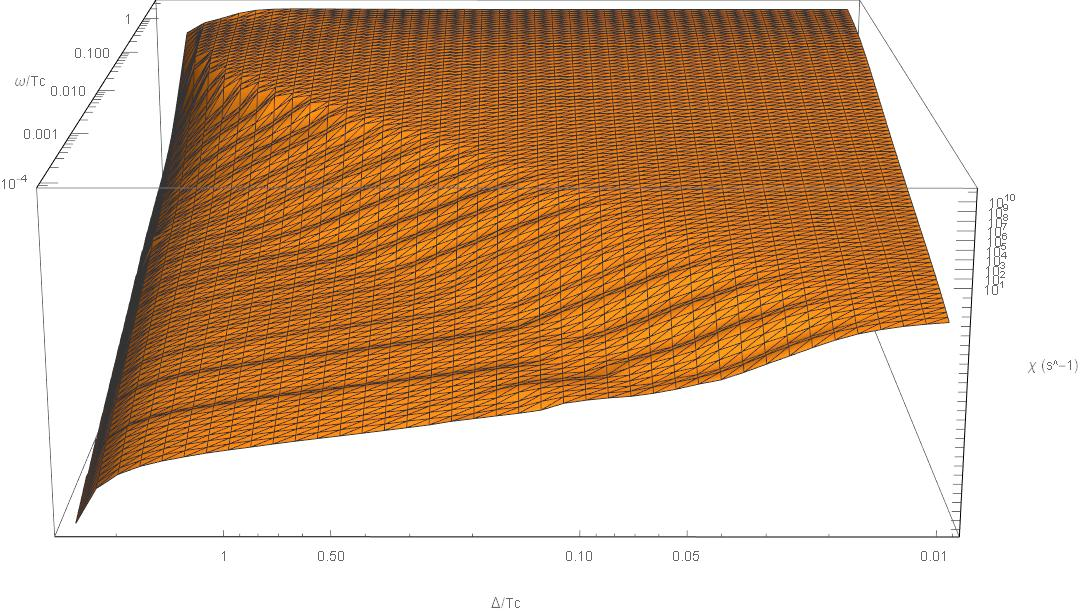
\includegraphics[width=\linewidth]{namNoiseCliff}
	\caption{$\chi = \frac{1}{T_1(z)}$ for fixed $z$, but varying $\omega$ and $\Delta$} \label{fig:Cliff}
\end{figure}
This is plotted in \cref{fig:Cliff}, which shows the cliff-edge along which $\omega$ is sufficiently smaller than $\Delta$.
In this regime, Johnson noise no longer becomes an issue for these qubits.

\subsection{Fitting the cliff}

We are interested in characterising the $\Delta$-$\omega$ curve that shows where the superconducting low-noise behaviour gives way to the normal state high-noise behaviour.
\Cref{fig:cliffview} shows the cliff in the computation we've been looking at, filtered to only include $\tau$ large enough to make the material look clean.

\begin{figure}[htp]
	\centering
	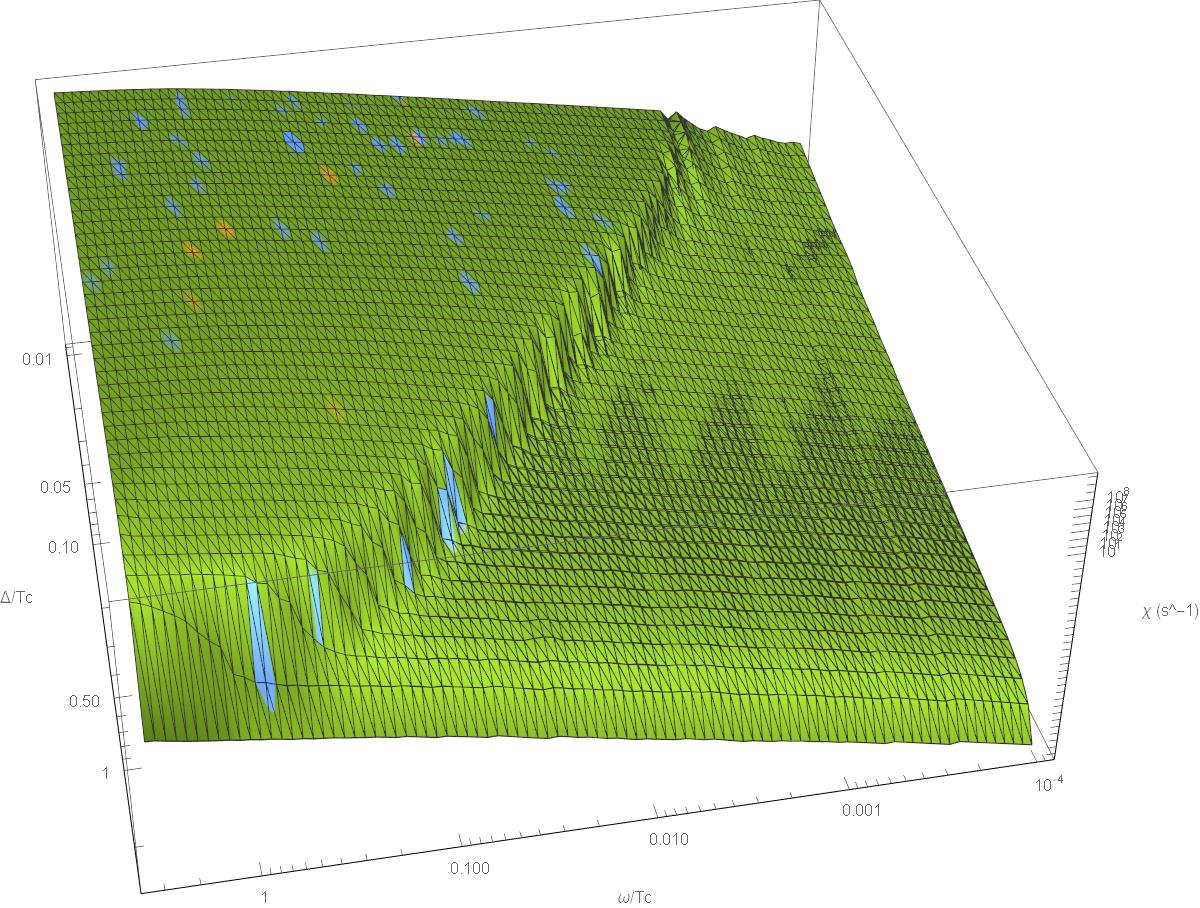
\includegraphics[width=\linewidth]{sharpcliffview}
	\caption{A view of the cliff for clean materials only} \label{fig:cliffview}
\end{figure}

\begin{figure}[htp]
	\centering
	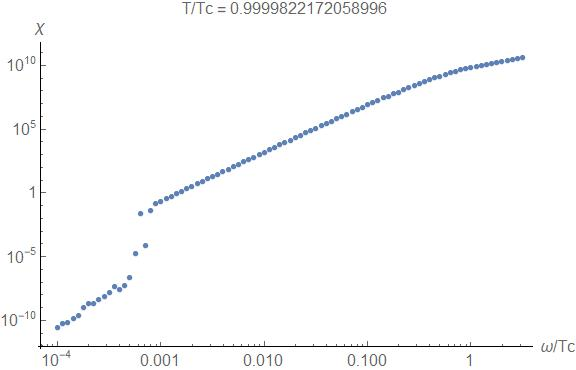
\includegraphics[width=\linewidth]{exampleconsttplot}
	\caption{An example slice of the 3D plot for constant temperature} \label{fig:exConstTPlot}
\end{figure}

\Cref{fig:exConstTPlot} shows a slice of \cref{fig:cliffview} for constant temperature.
In it the cliff is visible as the jump around $\frac{\omega}{T_c} \approx 0.001$.
Because \cref{fig:exConstTPlot} is plotted for a relatively high temperature, the $\omega$ at which the cliff occurs is low compared to $T_c$;
for lower temperatures the cliff would occur at higher frequencies.

We can demarcate the lower boundary of this cliff as the lowest frequency at which there is a discontinuity in the derivative of the log-log plot.
This is plotted in \cref{fig:exConstTPlotWithLine}.

\begin{figure}[htp]
	\centering
	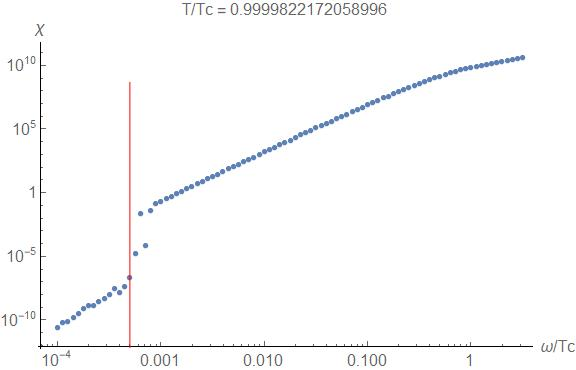
\includegraphics[width=\linewidth]{exampleconsttplotwithline}
	\caption{\Cref{fig:exConstTPlot} with a line showing the lower boundary of the cliff.} \label{fig:exConstTPlotWithLine}
\end{figure}

By iterating this process over all $T$, we can estimate the function $\omega_{lc}(T)$.
Lastly, we are really interested in the function $\omega_{lc}(\Delta)$, so we use $\frac{\Delta}{T_c} = 3.06 \sqrt{1 - t}$.

% TODO This plot is a little bit bad because of the multiple tau so clean that up in future plot.
\begin{figure}[htp]
	\centering
	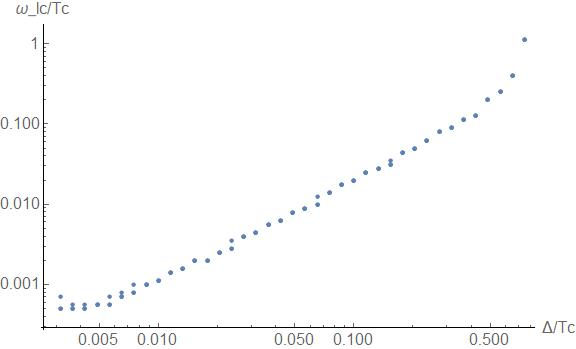
\includegraphics[width=\linewidth]{cleancliff}
	\caption{The points $\omega_lc(\Delta)$ estimated to be the bottom edge of the cliff.} \label{fig:cleancliff}
\end{figure}

We can see in \cref{fig:cleancliff} that the cliff does not follow a simple power law near the highest and lowest $\Delta$, but appears to do so for intermediate values of $\Delta$.
% TODO rewrite this to be more precise. the cluster process in the notes is probably insufficiently good on its own, but should be easy to clean up.
Fitting the expression $\omega_lc = A \Delta^B$ on only the central portion of \cref{fig:cleancliff} returns parameter values
\begin{align} %Todd because I got lazy with Delta this is technically slightly wrong, but easy to clean up later.
	A &= 0.452107 \\
	B &= 1.34246.
\end{align}

This expression is plotted in \cref{fig:fittedcliff}, as the curve in blue.
Intruigingly, the exponent $B$ is nearly the simple fraction $\frac{4}{3}$.
%Todo think about this

\begin{figure}[htp]
	\centering
	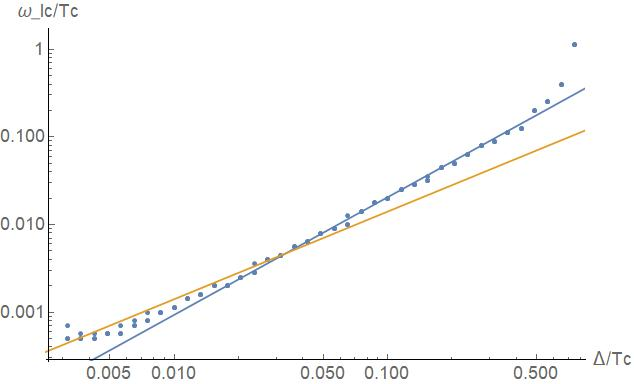
\includegraphics[width=\linewidth]{fittedcliff}
	\caption{\Cref{fig:cleancliff} with fits, described in the text of the notes.} \label{fig:fittedcliff}
\end{figure}


\section{Non-equilibrium state} \label{sec:nonequilibrium}
We must calculate the superconducting gap in the case where a material is kept out of equilibrium by quasiparticle injection.
This quasiparticle injection occurs via multiple physical mechanisms, such as shining photons on a superconducting surface as in Gao et. al\cite{Gao2008}, or applying a bias voltage as studied in Catelani et. al\cite{Catelani2010}.
Both Gao and Catelani obtain via different methods results analogous to Owen and Scalapino\cite{OwenScalapino}, which we summarise here.
% TODO Revisit with more detail about how Catelani is probably a more rigorous derivation of the OS results.

Owen and Scalapino derive the usual BCS gap equation, but by constraining quasiparticle number end up with an effective quasiparticle distribution function
\begin{equation}
	f_k = \frac{1}{1 + \exp[\beta \left(E_k - \corr \right)]}.
\end{equation}
This results in a modified gap equation:% TODO Maybe add more derivation so that people don't have to go back to BCS to understand.
\begin{equation}
	\left[ N(0) V \right]^{-1} = \int_{- \omega_D}^{\omega_D} \frac{\dd{\epsilon_k}}{\sqrt{\Delta^2 + \epsilon_k^2}} \tanh{\frac{\sqrt{\Delta^2 + \epsilon_k^2} - \corr}{2 T}}. \label{eq:gap}
\end{equation}
Owen and Scalapino also characterise the excess quasiparticle density $n$ in units of $4 N(0) \Delta_0$:
\begin{equation}
	n = \frac{1}{\Delta_0} \int_0^\infty \dd{\epsilon} \left( \frac{1}{1 + \exp(\frac{\sqrt{\Delta^2 + \epsilon_k^2} - \corr}{T})} - \frac{1}{1 + \exp(\frac{\sqrt{\Delta^2 + \epsilon_k^2}}{T})} \right). \label{eq:n}
\end{equation}

We are going to be interested in the case where we have a fixed $n$. % Todo expand on this%
This means that \eqref{eq:gap} and \eqref{eq:n} form two coupled integral equations in $\Delta$ and $\corr$, to be solved numerically.
\Cref{fig:osFig1Reproduction} plots $\Delta(T)$ for different $n$, mirroring Figure 1 in Owen and Scalapino\cite{OwenScalapino}. % todo replace with cleaner plot that doesn't have the nonphysical section%.

\begin{figure}[b]
	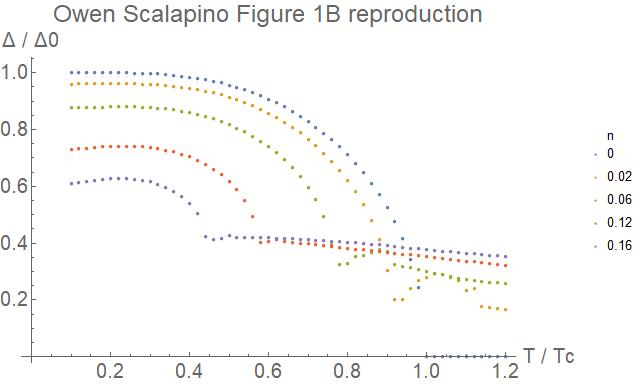
\includegraphics[width=\linewidth]{osGapVsTReproduction}
	\caption{\label{fig:osFig1Reproduction} Unitless $\Delta(T)$ for different $n$, calculated for $N(0)V = 0.2$ and $\debye = 100$ \cite{OwenScalapino}.}
\end{figure}

These results are constrained further by the material's energetics;
as Owen and Scalapino discuss, the solutions of \eqref{eq:gap} and \eqref{eq:n} may not be energetically favourable, and for increasing $n$ the critical temperature $T_c(n)$ will decrease.\cite{OwenScalapino}
Determining this decrease requires a model of the particular method by which the quasiparticle injection occurs, as the normal state free energy may change as well.
However, here we use Owen and Scalapino's approximate relation $T_c(n) \approx (1 - 4n) T_c(n = 0)$, as that is sufficiently descriptive for this study.

\subsection{Electromagnetic response}
To find the noise outside the surface, we must find the electromagnetic response function of the superconductor using the gap found above.
Because we are interested in a wide range of impurity concentrations in the supercondcutor, we use the electromagnetic response function first derived by Nam\cite{Nam1967}, which extends the previous models by Mattis and Bardeen~\cite{Mattis} and Abrikosov, Dzyaloshinskii and Gorkov\cite{AGD}.

The response function in Nam depends on the material's plasma frequency $\omega_p$, an impurity collision frequency $\tau$, the Fermi velocity $\vf$, and the gap $\Delta$.
For our noise calculation, we will need this function over the Fourier momentum $q$ and frequency $\omega$.
To simplify the notation, we define the following dimensionless quantities, keeping the variable $\mu$:
\begin{align}
	\xi &= \frac{\omega}{\Delta} \\
	\xi' &= \frac{\omega'}{\Delta} \\
	\nu &= \frac{1}{\tau \Delta} \\
	\kappa &= \frac{q \vf}{\Delta} \\
	t &= \frac{T}{\Delta} \\
	\sigma_0 &= \frac{n e^2}{m \Delta} \\
	\mu &= \frac{\corr}{\Delta}
\end{align}
Because our model includes modified quasiparticle distribution functions, we must modify these terms in the response function as well as the gap.
These appear in the $\tanh$ functions as an effective chemical potential. % TODO Write this out a bit more, sketching out the actual derivation.
Then the expression for the conductivity at arbitrary momentum and frequency in Nam\cite{Nam1967}, with the modified distribution function, becomes:
\begin{equation}
	\sigma(\kappa, \xi) = -i \frac{3 \sigma_0}{4} \frac{1}{\xi}\left[\int_{1 - \xi}^{1}\dd{\xi} \tanh(\frac{\xi + \xi' - \mu}{2 t}) I_1 + \int_{1}^{\infty} \dd{\xi'} \left( \tanh(\frac{\xi + \xi' - \mu}{2t}) I_1  - \tanh(\frac{\xi' - \mu}{2t})I_2 \right) \right] \label{eq:nonequilibrium:nam}
\end{equation}
with
\begin{align}
	I_1 &= F(\kappa, \Re[\sqrt{(\xi + \xi')^2 - 1} - \sqrt{\xi'^2 - 1}]) (g + 1) \nonumber\\
	&\quad + F(\kappa, \Re[-\sqrt{(\xi + \xi')^2 - 1} - \sqrt{\xi'^2 - 1}]) (g - 1) \\
	I_2 &= F(\kappa, \Re[\sqrt{(\xi + \xi')^2 - 1} - \sqrt{\xi'^2 - 1}]) (g + 1) \nonumber\\
	&\quad + F(\kappa, \Re[\sqrt{(\xi + \xi')^2 - 1} + \sqrt{\xi'^2 - 1}]) (g - 1) \\
	F(\kappa, E) &= \frac{1}{\kappa} \left[2 S(E) + (1 - S(E)^2)\ln(\frac{S(E) + 1}{S(E) - 1})\right]  \\
	S(\kappa, E) &= \frac{1}{\kappa} \left(E - i \left(\Im[\sqrt{(\xi + \xi')^2 - 1} + \sqrt{\xi'^2 - 1}] + 2 \nu \right) \right) \\
	g  &= \frac{\xi' \left( \xi + \xi'\right) + 1}{\sqrt{\xi'^2 - 1}\sqrt{(\xi + \xi')^2 - 1}}
\end{align}
We note here the similarity between \eqref{eq:nonequilibrium:nam} and the response functions in Catelini et. al\cite{Catelani2010}.

\section{Conclusion} \label{sec:conclusion}

\bibliography{bibliography}

\end{document}
